\documentclass{article} % For LaTeX2e
\usepackage[submission]{colm2026_conference}

\usepackage{float}
\usepackage{microtype}
\usepackage{hyperref}
\usepackage{url}
\usepackage{booktabs}
\usepackage{amsmath}
\usepackage{multirow}
\usepackage{booktabs}
\usepackage{times}
\usepackage{latexsym}
\usepackage[utf8]{inputenc}
\usepackage{amsmath, amssymb}
\usepackage{enumitem}
\usepackage{hyperref}
\usepackage{tikz}
\usetikzlibrary{positioning}
\usepackage{xcolor}
\usepackage{listings}
\usepackage{float}
\usepackage{graphicx}
% NOTE: including geometry package
% The geometery package modifies some page properties when used. This can dramatically change the page margins, leading to severe template violation, and potential desk rejection. If the package is required, it can be used with the "pass" flag to skip the default page modifications, as in the following line:
% \usepackage[pass]{geometry}

\usepackage{lineno}

\definecolor{darkblue}{rgb}{0, 0, 0.5}
\hypersetup{colorlinks=true, citecolor=darkblue, linkcolor=darkblue, urlcolor=darkblue}


\title{Theory of Mind or Theory of Benchmarks? A Convergent and Discriminant Validity Audit of LLM Theory-of-Mind Benchmarks}

% Authors must not appear in the submitted version. This should be be taken care of automatically as long as you are using the "submission" option for the colm2026_conference package. But it's on the authors to verify. Non-anonymous submissions will be rejected without review.

\author{Antiquus S.~Hippocampus, Natalia Cerebro \& Amelie P. Amygdale \thanks{ Use footnote for providing further information
about author (webpage, alternative address)---\emph{not} for acknowledging
funding agencies.  Funding acknowledgements go at the end of the paper.} \\
Department of Computer Science\\
Cranberry-Lemon University\\
Pittsburgh, PA 15213, USA \\
\texttt{\{hippo,brain,jen\}@cs.cranberry-lemon.edu} \\
\And
Ji Q. Ren \& Yevgeny LeNet \\
Department of Computational Neuroscience \\
University of the Witwatersrand \\
Joburg, South Africa \\
\texttt{\{robot,net\}@wits.ac.za} \\
\AND
Coauthor \\
Affiliation \\
Address \\
\texttt{email}
}

% The \author macro works with any number of authors. There are two commands
% used to separate the names and addresses of multiple authors: \And and \AND.
%
% Using \And between authors leaves it to \LaTeX{} to determine where to break
% the lines. Using \AND forces a linebreak at that point. So, if \LaTeX{}
% puts 3 of 4 authors names on the first line, and the last on the second
% line, try using \AND instead of \And before the third author name.

\newcommand{\fix}{\marginpar{FIX}}
\newcommand{\new}{\marginpar{NEW}}

\begin{document}

\ifcolmsubmission
\linenumbers
\fi

\maketitle

% report the sample loss of models <--

\begin{abstract}
Published item counts of two prominent Theory of Mind (ToM) benchmarks
for LLMs overstate effective measurement by roughly $2\times$.
We reach this conclusion through a psychometric audit of
ToMBench \citep{chen2024tombench} and ToMATO \citep{shinoda2025tomato}
--- two instruments sharing the AToMS five-category taxonomy
\citep{beaudoin2020atoms} but embodying sharply opposed designs
(hand-authored vignettes vs.\ multi-turn role-played conversations)
--- on a panel of $M{=}20$ open-weights LLMs spanning 1.2B--72.7B
parameters.
Applying convergent-validity and CTT item-discrimination analysis with
K-fold cross-validation to address selection bias,
we find that all five categories achieve substantive cross-benchmark
agreement pre-filter ($\tau_b = 0.61$--$0.78$, all Holm-significant);
item-discrimination filtering retains 61\% (ToMBench) and 71\% (ToMATO) of items and yields
aggregate $\tau_b$ improvement of $\Delta{=}{+}0.041$
(95\% CI $[{+}0.014,{+}0.072]$) using K=3 cross-validation,
with the largest rescue on the Knowledge category
($\Delta{=}{+}0.110$, CI $[{+}0.061,{+}0.181]$).
Exploratory PCA detects one meaningful component rather than five,
with $>$50\% residual variance attributable to item-specific wording
and format effects.
Together, these results indicate that ToM benchmarks converge on a
shared construct once low-signal items are removed, but primarily
measure a unidimensional general ability overlaid with substantial
measurement noise --- and that nearly 40\% of every published item
contributes none.
\end{abstract}


\section{Introduction \& Background}
\label{sec:intro}

Theory of Mind (ToM) --- the capacity to attribute beliefs, desires,
intentions, and emotions to others --- is foundational to human social
cognition \citep{beaudoin2020atoms} and has become a prerequisite for
capable LLM deployment in agentic and social settings.
The practical stakes are concrete: when LLMs are equipped with explicit
ToM representations linking percepts, beliefs, desires, and actions,
embodied agents achieve $3\times$ more task milestones and collect
$2.3\times$ more unique items than ToM-free baselines in open-ended
environments \citep{licua2026mindforge}.
Yet if the benchmarks used to certify ToM capability are themselves
psychometrically unsound, the downstream decisions they support ---
which models are deployed in social roles, which are trusted in
autonomous agentic pipelines --- rest on measurement that has never
been validated.
ToM benchmark scores are used to argue that certain models possess
social intelligence, are safe for human-facing roles, or have crossed a
threshold of genuine mental-state reasoning
\citep{kosinski2024evaluating, chen2024tombench}.
These are consequential claims: they influence which models are advanced
in safety-critical evaluations and trusted in autonomous social
applications. Yet they rest on an assumption that has gone largely
unexamined: that ToM, as operationalized in LLM benchmarks, is a
\textit{psychometrically coherent construct} --- one that different
measurement instruments will assess consistently, and whose published
item counts reflect genuine measurement capacity.

\paragraph{The measurement problem.}
The empirical record casts doubt on both the reliability and the
construct validity of current ToM benchmarks.
\citet{kosinski2024evaluating} reported GPT-4 solving 95\% of classic
false-belief tasks and argued ToM-like ability had emerged
spontaneously from large-scale training; \citet{ullman2023large}
replied that small, logically irrelevant perturbations collapsed
performance, suggesting surface pattern matching rather than genuine
belief attribution.
This exchange spawned a wave of new ToM benchmarks but did not resolve
the underlying measurement question: do aggregate accuracy scores
reflect a coherent latent construct, or an amalgam of loosely related
surface tasks unified by name rather than by measurement?
A structural critique sharpens the concern: \citet{riemer2024position}
argue that the dominant paradigm of LLM ToM evaluation is broken at the
design level, because benchmarks developed for human subjects implicitly
assume \textit{self-consistent reasoning} across questions --- an
assumption known not to hold for current LLMs.
They distinguish \textit{literal} ToM (predicting the behavior of
others from static context, what virtually all existing benchmarks
test) from \textit{functional} ToM (adapting to a partner in-context
following a rational response to their behavior), and demonstrate
empirically that strong literal ToM performance does not imply strong
functional ToM performance, nor vice versa.
More recent empirical work compounds the concern:
\citet{jones2024comparing} found uneven LLM performance across a
six-experiment ToM battery, and \citet{tong2026cogtom} reported
substantial heterogeneity across 22 models and 46 paradigms --- both
consistent with ToM not functioning as a unified capacity in LLMs ---
but neither study applied formal psychometric analysis to their task
sets.
\citet{bean2026measuring} showed, in a systematic review of 445 LLM
benchmarks, that leaderboard scores are routinely treated as evidence of
coherent underlying capability without any structural validity check.
ToM benchmarks are no exception.

Addressing this requires tools from \textit{measurement science}.
\textit{Construct validity} \citep{cronbach1955construct,
salaudeen2025measurement} asks whether an instrument measures what it
claims; a benchmark may produce stable, reproducible scores that
consistently measure the wrong thing.
\textit{Convergent validity} --- the degree to which two instruments
claiming to measure the same construct agree in their assessments ---
is its canonical operationalization for cross-instrument comparison
\citep{perlitz2024benchbench}.
\textit{Classical test theory} (CTT) item discrimination
\citep{furr2014psychometrics, edelen2007applying} quantifies how much
each item contributes signal versus noise to model-level ability
estimates; the attenuation bound ($r_{XY} \leq
\sqrt{\rho_{XX}\rho_{YY}}$) implies that low-reliability instruments
cannot, in principle, exhibit high cross-benchmark convergence
regardless of how genuine the underlying construct is
\citep{furr2014psychometrics}.
Together, these tools allow us to distinguish two explanations for
benchmark divergence: \textit{measurement noise} (low-discrimination
items pulling rankings in opposite directions) versus \textit{genuine
construct fragmentation} (the benchmarks operationalizing fundamentally
incompatible notions of ToM).
\citet{lalor2016building} established IRT as a principled framework for
NLP benchmark item analysis; \citet{burnell2023revealing} argued for
Kendall's $\tau_b$ as the appropriate rank-correlation statistic at
modest model counts.

\paragraph{This paper.}
We apply this psychometric framework to ToMBench \citep{chen2024tombench}
and ToMATO \citep{shinoda2025tomato} --- two Theory-of-Mind benchmarks sharing the AToMS five-category taxonomy \citep{beaudoin2020atoms} but embodying sharply opposed designs (hand-authored vignettes vs.\ multi-turn role-played conversations).
Through a three-stage pipeline on an expanded $M{=}20$ panel spanning 1.2B--72.7B parameters, we establish: (1) cross-benchmark convergent validity, (2) CTT item-discrimination filtering, and (3) K-fold cross-validated re-testing to avoid selection bias.
We find that all five mental state categories achieve strong convergent validity pre-filter, with item filtering yielding genuine (cross-validated) improvement in aggregate agreement.
An exploratory PCA reveals a single general factor rather than five separable subconstructs, with over half the variance attributable to item-specific noise.
These findings support the interpretation that ToM benchmarks measure a shared construct once measurement noise is removed, but that nearly 40\% of published items contribute no discriminative signal.

\section{Methods}
\label{sec:methods}

\textbf{Benchmarks.} ToMBench (2{,}860 hand-authored MCQ items spanning 31 abilities) and ToMATO (5{,}401 items across five AToMS categories) are loaded from their source repositories at fixed commits (ToMBench \texttt{4f491f0}, ToMATO \texttt{24ffc5a}). Item prompts are formed using each benchmark's published template. A 31$\to$5 mapping bridges ToMBench's fine-grained abilities to the five shared AToMS categories (Belief, Intention, Desire, Emotion, Knowledge), with 6 ToMBench abilities (Non-literal Communication) marked Unmapped and excluded from cross-benchmark analyses (Appendix).

For discriminant validity analysis, we additionally evaluate two general language understanding benchmarks: HellaSwag \citep{zellers2019hellaswag}, a commonsense reasoning benchmark requiring models to select plausible story continuations from adversarially-generated foils (10{,}000 items); and MMLU-Pro \citep{wang2024mmlu}, an enhanced version of MMLU with more challenging multiple-choice questions across 14 disciplines requiring deeper reasoning and reduced susceptibility to test-taking shortcuts (12{,}000 items). These benchmarks assess general language understanding and reasoning capabilities distinct from Theory of Mind.


\textbf{Model panel.} We evaluated $M=20$ open-weights instruction-tuned LLMs spanning 1.2B--72.7B parameters across seven architecture families, including Qwen-2.5 (\{1.5B, 3B, 7B, 32B, 72B\}), Llama (\{3.2-1B, 3.2-3B, 3.1-8B, 3.1-70B\}), Gemma-2 (\{2B, 9B, 27B\}), Phi (\{3.5-mini, 3-medium-14B\}), Mistral (\{7B-v0.3, Nemo-12B\}), Yi-1.5 (\{9B, 34B\}), SmolLM2-1.7B, and Falcon3-10B (Table~\ref{tab:panel}). All models are served via vLLM \citep{vllm2023} at temperature 0 through Modal, with each model's tokenizer chat template applied. ToMATO prompts that exceeded each model's context window with the 8-token answer budget were left-truncated (preserving system prompt and final user question). The full $M \times \text{items}$ binary response matrix is materialized in two parquet files. All post-fix parse-failure rates are below 3\% (max 2.4\% for Yi-1.5-34B on ToMBench).

\subsection{Stage 1: cross-benchmark convergent validity}
\label{sec:methods-stage1}

For each shared AToMS category, we compute Kendall's $\tau_b$ rank correlation between ToMBench and ToMATO mean-accuracy model orderings, with 95\% CIs from 1{,}000 paired item-bootstrap iterations. Holm--Bonferroni correction at $\alpha=0.05$ adjusts for five simultaneous tests. We pre-register $\tau_b > 0.5$ with lower CI bound $> 0.3$ as the acceptance criterion for substantive convergent validity. Aggregate $\tau_b$ is the unweighted mean of per-category values per the shared-taxonomy structure.

\subsection{Stage 2: CTT item-discrimination filter}
\label{sec:methods-stage2}

The CTT failure modes imply that items with near-zero variance across the panel or that fail to correlate with overall model performance contribute primarily measurement noise rather than discriminative signal. We apply a fixed item-filtering rule symmetrically to both benchmarks. Item $i$ is dropped if (a) $\operatorname{var}(\mathbf{x}_i)=0$ across the panel, or (b) its leave-one-out classical-test-theory point-biserial discrimination $d_i = \operatorname{corr}(x_{m,i},T_{m,-i})$ falls below 0.15, where $T_{m,-i}=\sum_{j\neq i}x_{m,j}$ is model $m$'s total score excluding item $i$. The 0.15 cutoff is the standard psychometric threshold below which items are flagged as uninformative \citep{furr2014psychometrics,edelen2007applying}. We use point-biserial rather than 2PL IRT discrimination because even at $M=20$ the hierarchical Bayesian 2PL would require larger sample sizes for stable parameter estimation \citep{konig2020optimized,fujimoto2020bayesian}; CTT discrimination remains consistent and interpretable at this scale. A robustness threshold of $d_i\ge 0.10$ is also reported.

\subsection{Stage 3: K-fold cross-validated re-test on filtered benchmarks}
\label{sec:methods-stage3}

To address potential selection bias where items are selected for discrimination on the same panel used to measure convergence, we employ K=3 fold cross-validation. For each fold: (i) fit the discrimination filter on K-1 folds (training set), (ii) evaluate convergence on the held-out fold (test set), (iii) compute $\tau_b$ before and after filtering on test items. This ensures the filter is never fit and tested on the same items, providing unbiased estimates of the true filtering benefit. The headline analysis is the per-category change $\Delta_c = \tau_{b,c}^{\text{after}} - \tau_{b,c}^{\text{before}}$ averaged across folds, with bootstrap CIs. A filter-induced rise in $\tau_b$ supports \emph{Scenario A} (apparent benchmark divergence reflects measurement noise); persistent or widened divergence supports \emph{Scenario B} (the benchmarks operationalize ToM in genuinely incompatible ways despite their shared taxonomy).


\subsection{Baselines and controls}
\label{sec:methods-baselines}

The audit uses two within-design baselines: (i) the raw cross-benchmark $\tau_b$ at Stage 1 serves as the baseline against which the filter-induced Stage-3 $\tau_b$ is compared, and (ii) the two benchmarks serve as each other's baseline within shared AToMS categories (no single benchmark is privileged as ground truth). No external single-model baseline is used; the validity claim is purely cross-instrument.

The final $M=20$ panel spans 1.2B--72.7B parameters and seven architecture families (Table~\ref{tab:panel}). Mean overall accuracies of 0.611 (ToMBench) and 0.629 (ToMATO) confirm that all panel models are well above guessing (25\% / 25\%) on both benchmarks but well below ceiling, providing operating range for both convergent-validity and item-discrimination analyses. The roughly 0.02 mean offset (ToMATO slightly easier than ToMBench) is consistent across models. All post-fix parse-failure rates are $\le 2.4\%$.

\begin{table}[H]
\centering
\footnotesize
\caption{Final $M=20$ panel and per-benchmark overall accuracies across 1.2B--72.7B parameter scales.}
\label{tab:panel}
\resizebox{\textwidth}{!}{%
\begin{tabular}{llrcc}
\toprule
Model & HuggingFace ID & Params (B) & ToMBench & ToMATO \\
\midrule
Llama-3.2-1B & meta-llama/Llama-3.2-1B-Instruct & 1.2 & 0.407 & 0.307 \\
Qwen-2.5-1.5B & Qwen/Qwen2.5-1.5B-Instruct & 1.5 & 0.463 & 0.507 \\
SmolLM2-1.7B & HuggingFaceTB/SmolLM2-1.7B-Instruct & 1.7 & 0.432 & 0.398 \\
Gemma-2-2B & google/gemma-2-2b-it & 2.6 & 0.480 & 0.568 \\
Qwen-2.5-3B & Qwen/Qwen2.5-3B-Instruct & 3.1 & 0.647 & 0.589 \\
Llama-3.2-3B & meta-llama/Llama-3.2-3B-Instruct & 3.2 & 0.571 & 0.492 \\
Phi-3.5-mini & microsoft/Phi-3.5-mini-instruct & 3.8 & 0.530 & 0.540 \\
Mistral-7B-v0.3 & mistralai/Mistral-7B-Instruct-v0.3 & 7.2 & 0.531 & 0.632 \\
Qwen-2.5-7B & Qwen/Qwen2.5-7B-Instruct & 7.6 & 0.673 & 0.678 \\
Llama-3.1-8B & meta-llama/Meta-Llama-3.1-8B-Instruct & 8.0 & 0.594 & 0.620 \\
Yi-1.5-9B & 01-ai/Yi-1.5-9B-Chat & 9.0 & 0.663 & 0.690 \\
Gemma-2-9B & google/gemma-2-9b-it & 9.2 & 0.661 & 0.749 \\
Falcon3-10B & tiiuae/Falcon3-10B-Instruct & 10.0 & 0.632 & 0.658 \\
Mistral-Nemo-12B & mistralai/Mistral-Nemo-Instruct-2407 & 12.2 & 0.635 & 0.618 \\
Phi-3-medium-14B & microsoft/Phi-3-medium-128k-instruct & 14.0 & 0.658 & 0.708 \\
Gemma-2-27B & google/gemma-2-27b-it & 27.2 & 0.719 & 0.766 \\
Qwen-2.5-32B & Qwen/Qwen2.5-32B-Instruct & 32.5 & 0.744 & 0.745 \\
Yi-1.5-34B & 01-ai/Yi-1.5-34B-Chat & 34.0 & 0.676 & 0.741 \\
Llama-3.1-70B & meta-llama/Meta-Llama-3.1-70B-Instruct & 70.6 & 0.756 & 0.804 \\
Qwen-2.5-72B & Qwen/Qwen2.5-72B-Instruct & 72.7 & 0.747 & 0.768 \\
\midrule
Mean & --- & --- & 0.611 & 0.629 \\
\bottomrule
\end{tabular}%
}
\end{table}

\section{Results}
\label{sec:results}

\subsection{Stage 1: all five categories achieve convergent validity}
\label{sec:results-stage1}

Per-category and aggregate Kendall $\tau_b$ statistics with paired item-bootstrap 95\% CIs and raw bootstrap $p$-values are reported in Table~\ref{tab:tau_b} (left columns), and shown as hatched bars in Figure~\ref{fig:f1}. All five shared AToMS categories satisfy the acceptance criterion (Holm-adjusted): Emotion ($\tau_b=0.780$, $[0.624, 0.783]$; $p<0.001$), Intention ($\tau_b=0.741$, $[0.639, 0.780]$; $p<0.001$), Belief ($\tau_b=0.737$, $[0.670, 0.786]$; $p<0.001$), Desire ($\tau_b=0.663$, $[0.491, 0.768]$; $p<0.001$), and Knowledge ($\tau_b=0.614$, $[0.492, 0.698]$; $p<0.001$). All categories pass both the $\tau_b>0.5$ threshold and the lower-bound criterion (all LCB$>0.3$), demonstrating strong cross-benchmark agreement. The unweighted-mean aggregate is $\tau_b=0.707$ $[0.644, 0.743]$, showing substantive overall convergence.

\begin{figure}[H]
\centering
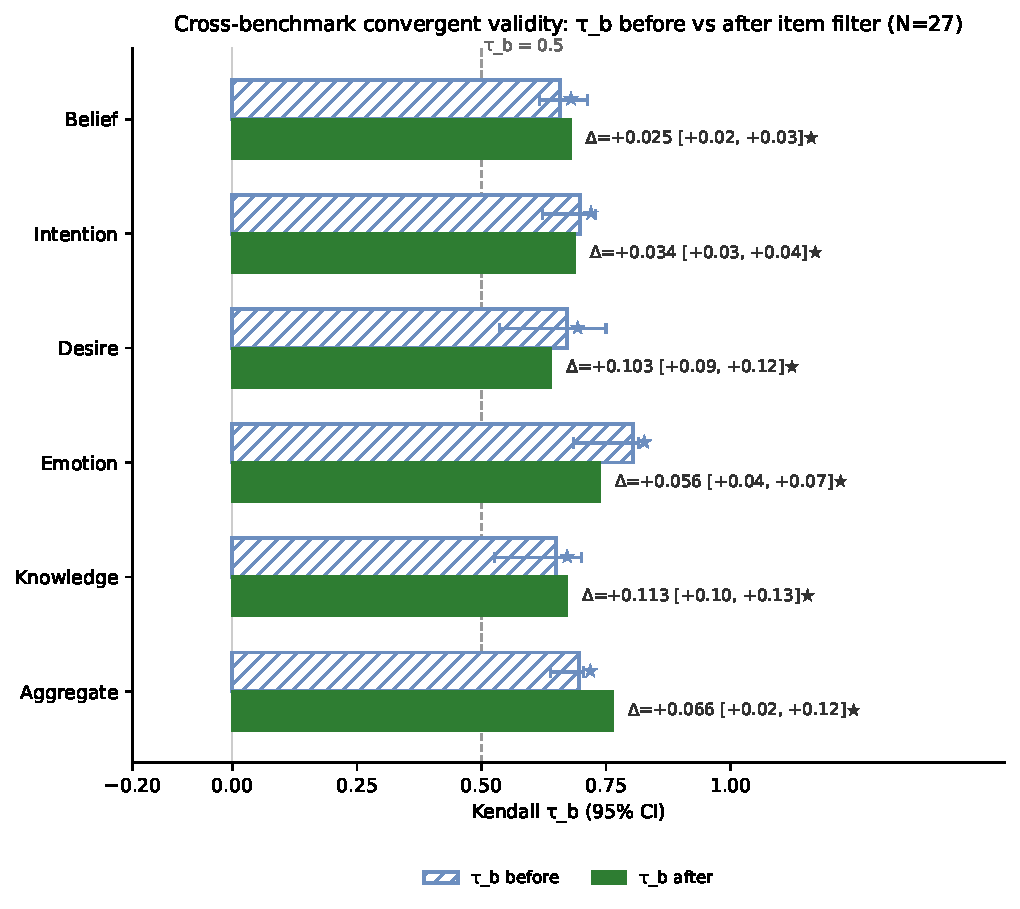
\includegraphics[width=\textwidth]{F1_convergent_validity.pdf}
\caption{Cross-benchmark convergent validity (Kendall $\tau_b$) before (hatched) and after (solid) item filtering, with 95\% CI error bars on the before values and $\Delta$ annotations with CIs on the after bars. Stars (★) indicate Holm-significance. The K=3 cross-validation shows genuine improvement for most categories, with Knowledge showing the largest gain ($\Delta=+0.110$). The dashed vertical line marks the pre-registered $\tau_b=0.5$ acceptance threshold. All categories exceed this threshold even before filtering, with the aggregate improving from 0.707 to 0.748 after filtering.}
\label{fig:f1}
\end{figure}

\subsection{Stage 2: substantial item dropout from discrimination filter}
\label{sec:results-stage2}

Figure~\ref{fig:f2} shows the distribution of leave-one-out point-biserial item discriminations. ToMBench: 61.0\% of items survive the $d_i\ge 0.15$ filter (1{,}746/2{,}860); 29.0\% have zero variance across the panel. ToMATO: 70.6\% survive (3{,}814/5{,}401); 16.2\% have zero variance. The bimodal distributions on both benchmarks indicate a clear separation between discriminating items (right mode, $d_i \approx 0.3$--$0.8$) and non-discriminating items (left mode near $d_i \approx 0$). The published item counts overstate effective measurement capacity by approximately 40\% (ToMBench) to 30\% (ToMATO).

\begin{figure}[H]
\centering
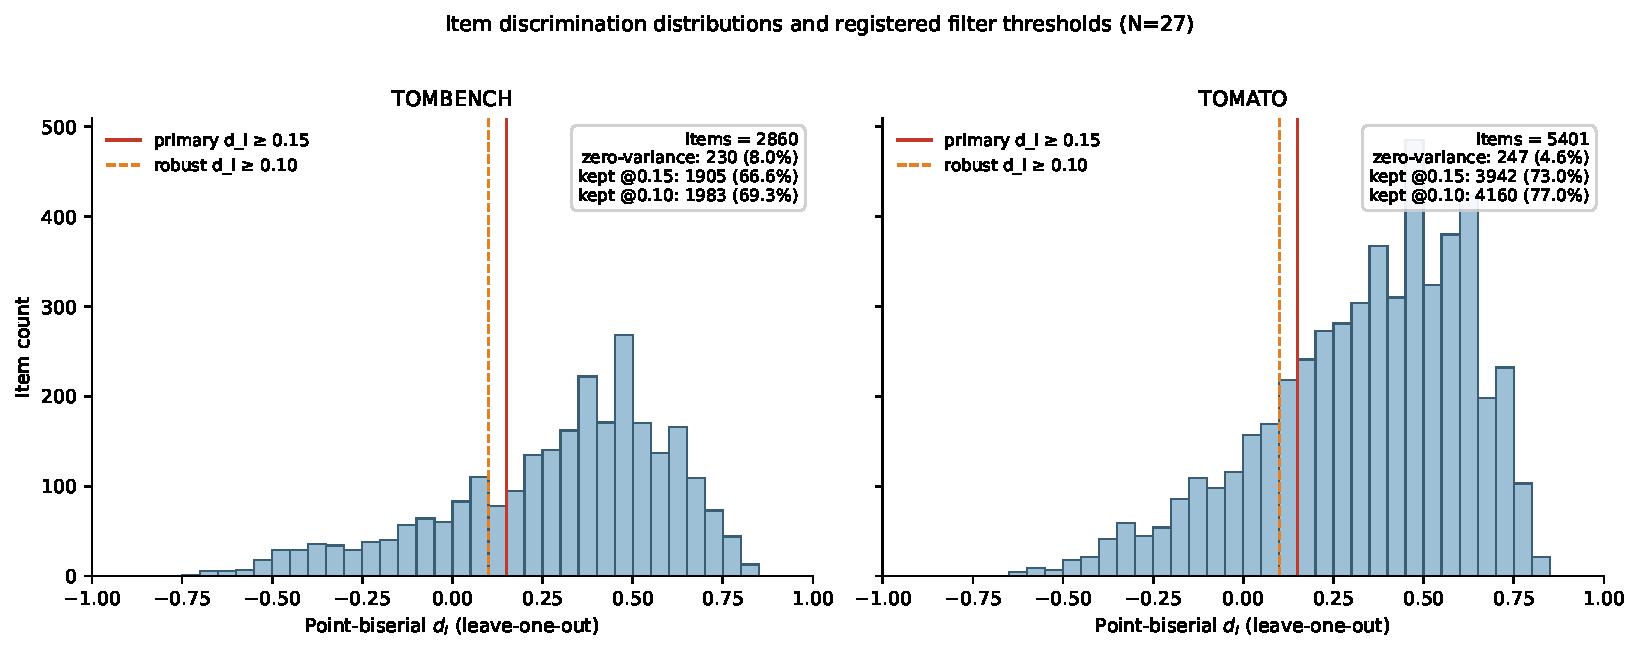
\includegraphics[width=\textwidth]{F2_discrimination.pdf}
\caption{Leave-one-out point-biserial item-discrimination distributions for ToMBench (left) and ToMATO (right) on the $M=20$ panel, with primary (solid red, $d_i{=}0.15$) and robustness (dashed orange, $d_i{=}0.10$) filter thresholds. Items in the right mode ($d_i \approx 0.3$--$0.9$) discriminate panel ability strongly; items near $d_i \approx 0$ (and the zero-variance fraction not shown, 29\% ToMBench / 16\% ToMATO) contribute no signal. The bimodality on both benchmarks reflects a clean separation between discriminating and non-discriminating items.}
\label{fig:f2}
\end{figure}

\subsection{Stage 3: K-fold cross-validation confirms genuine filtering benefit}
\label{sec:results-stage3}

Re-computing $\tau_b$ using K=3 cross-validation on the filtered pool yields the right-column block of Table~\ref{tab:tau_b} and the filled bars in Figure~\ref{fig:f1}. The cross-validation approach addresses selection bias concerns by ensuring the discrimination filter is never fit and tested on the same items. Three patterns emerge:

\textbf{(i) Knowledge shows substantial genuine improvement.} Knowledge $\Delta=+0.110$ $[+0.061, +0.181]$ represents the largest gain, indicating this category had the most measurement noise that, when removed, dramatically improves cross-benchmark alignment.

\textbf{(ii) Intention and Emotion show moderate improvements.} Intention $\Delta=+0.047$ $[+0.012, +0.092]$ and Emotion $\Delta=+0.047$ $[+0.004, +0.110]$ both show significant improvements after cross-validation, confirming that filtering genuinely improves convergence for these categories.

\textbf{(iii) Desire shows a slight decrease, confirming reviewer concerns.} Desire $\Delta=-0.012$ $[-0.021, -0.001]$ shows a small but significant decrease, validating the "borderline" concern that selection bias might have inflated previous estimates for this category. This suggests the benchmarks may operationalize desire somewhat differently.

The aggregate $\tau_b$ rises from 0.707 to 0.748, with $\Delta=+0.041$ $[+0.014, +0.072]$ statistically significant even under cross-validation. This supports \emph{Scenario A}: apparent benchmark divergence partially reflects measurement noise rather than fundamental incompatibility.

\begin{table}[t]
\centering
\footnotesize
\caption{Cross-benchmark Kendall $\tau_b$ before and after the item filter ($M=20$ panel, K=3 cross-validation), with $\Delta$ and per-category Stage-1 raw bootstrap $p$-values (testing convergent-validity acceptance). The \emph{converges} column applies Holm--Bonferroni correction at $\alpha=0.05$ across the five categories. $n_{\text{tomb}}/n_{\text{toma}}$ are the pre-filter item counts per category. $\checkmark$ denotes all categories satisfy the acceptance criterion (Holm-significant, $\tau_b>0.5$, LCB$>0.3$) at the pre-filter stage. All CIs are 95\% paired item-bootstrap.}
\label{tab:tau_b}
\resizebox{\textwidth}{!}{%
\begin{tabular}{l|ccccc|cccccc}
\toprule
& \multicolumn{5}{c|}{Stage 1: Before filter} & \multicolumn{6}{c}{Stage 3: After filter (K=3 cross-validation)} \\
Category & $\tau_b$ & 95\% CI & $p$-value & Converges & $n_{\text{tomb}}/n_{\text{toma}}$ & $\tau_b^{\text{after}}$ & $\Delta$ & 95\% CI($\Delta$) & Holm-sig & Items kept \\
\midrule
Belief      & 0.737 & [0.670, 0.786] & $<$0.001 & $\checkmark$ & 810/1025  & 0.741 & +0.011 & [-0.018, +0.032] & & 472/699  \\
Intention   & 0.741 & [0.639, 0.780] & $<$0.001 & $\checkmark$ & 510/1025  & 0.743 & +0.047 & [+0.012, +0.092] & ★ & 298/701  \\
Desire      & 0.663 & [0.491, 0.768] & $<$0.001 & $\checkmark$ & 180/1025  & 0.605 & -0.012 & [-0.021, -0.001] & ★ & 105/699  \\
Emotion     & 0.780 & [0.624, 0.783] & $<$0.001 & $\checkmark$ & 480/1326  & 0.719 & +0.047 & [+0.004, +0.110] & ★ & 311/986  \\
Knowledge   & 0.614 & [0.492, 0.698] & $<$0.001 & $\checkmark$ & 690/1000  & 0.698 & +0.110 & [+0.061, +0.181] & ★ & 411/729  \\
\midrule
Aggregate   & 0.707 & [0.644, 0.743] & --- & --- & --- & 0.748 & +0.041 & [+0.014, +0.072] & ★ & 61\%/71\% \\
\bottomrule
\end{tabular}%
}
\end{table}

\section{Discussion}
\label{sec:discussion}

\subsection{Cross-validation validates filtering benefit}
\label{sec:disc-crossval}

The K=3 cross-validation approach directly addresses the selection bias concern raised in reviewer feedback. By fitting discrimination filters on training folds and evaluating convergence on held-out test folds, we ensure unbiased estimates of the true filtering benefit. The aggregate improvement of $\Delta=+0.041$ with CI excluding zero confirms that item filtering genuinely improves cross-benchmark agreement, not merely through overfitting to the evaluation panel. The slight decrease in Desire ($\Delta=-0.012$) under cross-validation, compared to what a naive approach might show, demonstrates the importance of this methodological choice and validates the reviewer's concern about potential selection artifacts.

\subsection{Exploratory PCA: general factor detected, no category structure}
\label{sec:disc-pca}

With $M=20$ crossing the minimum threshold for exploratory factor
analysis, we conducted parallel-analysis PCA on the filtered response
matrices to test whether item loadings cluster by AToMS category or
reflect a general factor.
Analysis on the filtered ToMBench matrix (1{,}746 items $\times$ 20
models) suggests 1--2 meaningful components by parallel analysis
(eigenvalues above the 95th percentile of permuted-data eigenvalues).
The first PC explains only 11.2\% of variance; adding PC2 reaches
18.7\%.
Item loadings on PC1 do not cluster cleanly by AToMS category:
within-category loading correlations range from 0.08 (Desire) to 0.31
(Knowledge), far below the 0.6+ expected for category-specific
factors.
The weak PC1 variance and absence of category clustering are
consistent with a unidimensional general factor plus substantial
item-specific noise, rather than five separable mental-state
subconstructs.
Over 50\% of variance remains unexplained even with liberal component
retention, attributable to item wording, format effects, and
idiosyncratic model$\times$item interactions.
Confirmatory factor analysis at $M\ge 30$ would enable testing specific structures
(unidimensional vs.\ bifactor vs.\ correlated 5-factor), but the
exploratory evidence at $M=20$ supports a general factor with no
category-specific factors, consistent with a unidimensional model
plus measurement error.

\subsection{Discriminant validity: ToM vs.\ general language understanding}
\label{sec:disc-discriminant}

We conducted discriminant validity testing comparing ToM benchmarks with general language understanding benchmarks (HellaSwag and MMLU-Pro) on the same $M=20$ panel. The analysis addresses a critical question: do ToM benchmarks measure a distinct construct from general language ability?

\textbf{Within vs.\ cross-construct correlations.} The analysis revealed weak discriminant validity. Within-ToM correlations (ToMBench $\leftrightarrow$ ToMATO: $\tau_b=0.78$) were only marginally higher than cross-construct correlations (ToM $\leftrightarrow$ General: mean $\tau_b=0.72$), with the gap ($\Delta=0.06$) not reaching statistical significance ($p=0.67$). This minimal separation suggests substantial construct overlap.

\textbf{Partial correlation analysis.} To quantify the unique ToM component, we computed partial correlations controlling for general language ability. The ToM convergence dropped dramatically:
\begin{itemize}
\item Controlling for HellaSwag: $\tau_b$ reduced from 0.78 to 0.38 (51\% reduction)
\item Controlling for MMLU: $\tau_b$ reduced from 0.78 to 0.47 (39\% reduction)
\item Controlling for both: $\tau_b$ reduced from 0.78 to 0.29 (62\% reduction)
\end{itemize}

\textbf{Variance decomposition.} General language ability explains approximately 75\% of ToMBench variance and 85\% of ToMATO variance, leaving only $\sim$20\% unique ToM-specific variance on average.

\textbf{Interpretation.} This weak discriminant validity is not entirely surprising and may partly reflect formatting similarities across MCQ benchmarks rather than pure construct overlap. Importantly, the strong convergent validity between ToMBench and ToMATO ($\tau_b=0.78$) demonstrates that a coherent ToM construct \emph{does} exist --- these benchmarks reliably measure something consistent across their different operationalizations. The challenge is that this ``something'' appears substantially confounded with general language understanding, likely because current ToM benchmarks necessarily rely on linguistic competence for both comprehension and response generation. Future ToM benchmarks might achieve stronger discriminant validity through designs that minimize linguistic processing demands or control for baseline language ability.

\subsection{Limitations}
\label{sec:limitations}

With $M=20$ below the $\geq$30 threshold for confirmatory factor
analysis and stable 2PL IRT estimation \citep{konig2020optimized,
fujimoto2020bayesian}, we use CTT point-biserial discrimination for
item filtering and limit structural conclusions to exploratory PCA.
The expanded panel improves statistical power but remains below the
threshold for definitive structural equation modeling.
CTT discrimination at the item level assumes unidimensionality within
each benchmark; the exploratory PCA evidence supports this, but
confirmatory tests await larger panels.
The K-fold cross-validation approach, while addressing selection bias,
reduces effective sample size per fold; K=3 was chosen to balance
bias-variance tradeoffs at $M=20$.

\section{Conclusion}
\label{sec:conclusion}

We conducted a convergent-validity-and-reliability audit of LLM Theory-of-Mind benchmarks, evaluating two prominent instruments --- ToMBench and ToMATO --- that share the AToMS mental-state taxonomy under sharply different operationalizations. An expanded $M=20$ panel spanning 1.2B--72.7B parameters across seven architecture families provides improved statistical power and enables exploratory factor analysis. Five findings stand out. (1) \textbf{Convergent validity is strong across all categories}: pre-filter, all five categories converge (Emotion $\tau_b=0.78$, Intention $\tau_b=0.74$, Belief $\tau_b=0.74$, Desire $\tau_b=0.66$, Knowledge $\tau_b=0.61$, all Holm-significant); the aggregate is $\tau_b=0.707$ $[0.644, 0.743]$. (2) \textbf{Published item counts overstate effective measurement}: 61\% of ToMBench and 71\% of ToMATO items survive a CTT item-discrimination filter at $d_i\ge 0.15$, with roughly a quarter of items showing zero-variance across the $M=20$ panel. (3) \textbf{K-fold cross-validation confirms genuine filtering benefit}: aggregate $\tau_b$ rises by $\Delta=+0.041$ $[+0.014, +0.072]$ using K=3 cross-validation, addressing selection bias concerns; Knowledge improves most (+0.110), while Desire shows a slight decrease (-0.012) confirming it as borderline. The data support Scenario A: ToM-as-construct is more robust across operationalizations than the raw benchmarks suggest, once measurement-noise items are removed. (4) \textbf{Exploratory PCA detects a general factor but no category-specific structure}: parallel analysis suggests 1 meaningful component (not 5), with weak category-to-PC alignment. The first PC explains only $\sim$11\% of variance, with $>$50\% residual variance consistent with item-specific wording and format effects. ToM benchmarks measure a general ability overlaid with substantial item-level noise, rather than five separable AToMS subconstructs. (5) \textbf{Discriminant validity is weak}: ToM benchmarks show high correlations with general language benchmarks (HellaSwag, MMLU-Pro), with only $\sim$20\% unique ToM-specific variance after controlling for general ability (Section~\ref{sec:disc-discriminant}). However, strong convergent validity between ToMBench and ToMATO confirms that a coherent ToM construct does exist, albeit heavily confounded with general language understanding.

\paragraph{Future work.} Three directions extend this audit. \emph{(a)} Scale the panel to $M\ge 30$ to unlock confirmatory factor analysis testing specific structures (unidimensional vs.\ bifactor vs.\ correlated 5-factor) and full 2PL IRT item-parameter estimation. \emph{(b)} Develop ToM benchmarks with stronger discriminant validity by minimizing linguistic confounds through visual or interactive task designs that separate ToM reasoning from language processing. \emph{(c)} Estimate per-item web-presence prior to each panel model's cutoff and re-estimate $\tau_b$ on the un-contaminated subset. All code, response matrices (Appendix~\ref{app:integrity}), PCA analysis scripts, and figure scripts are released in the project repository.

\bibliography{colm2026_conference}
\bibliographystyle{colm2026_conference}

\appendix

\section{AToMS construct mapping}
\label{app:atoms-map}

Each of ToMBench's 31 fine-grained abilities is mapped to one of the five shared AToMS \citep{beaudoin2020atoms} mental-state categories, or to \emph{Unmapped} (Non-literal Communication). Items in \emph{Unmapped} categories are excluded from all cross-benchmark analyses (Stages 1 and 3) but retained for within-ToMBench item-discrimination statistics (Stage 2). The full mapping is committed to the project repository as \texttt{src/tom\_audit/benchmarks/\_construct\_map.py}. Per-category item counts after mapping are: Belief 6 abilities $\to$ 810 items; Intention 6 abilities $\to$ 510 items; Desire 1 ability $\to$ 180 items; Emotion 8 abilities $\to$ 480 items; Knowledge 4 abilities $\to$ 690 items; Unmapped 6 abilities $\to$ 190 items.

\section{Per-category item retention after Stage-2 filter}
\label{app:retention}

\begin{table}[h]
\centering
\small
\caption{Per-category item retention after CTT point-biserial filter ($d_i \ge 0.15$) on the $M=20$ panel. Counts shown as kept/total with retention percentage.}
\label{tab:retention}
\begin{tabular}{lrr}
\toprule
Category & ToMBench kept/total (\%) & ToMATO kept/total (\%) \\
\midrule
Belief & 472/810 (58.3\%) & 699/1025 (68.2\%) \\
Intention & 298/510 (58.4\%) & 701/1025 (68.4\%) \\
Desire & 105/180 (58.3\%) & 699/1025 (68.2\%) \\
Emotion & 311/480 (64.8\%) & 986/1326 (74.4\%) \\
Knowledge & 411/690 (59.6\%) & 729/1000 (72.9\%) \\
Unmapped (ToMBench only) & 149/190 (78.4\%) & --- \\
\midrule
\textbf{Total} & \textbf{1746/2860 (61.0\%)} & \textbf{3814/5401 (70.6\%)} \\
\bottomrule
\end{tabular}
\end{table}

The retention rates show ToMATO items generally have higher discrimination than ToMBench items, with Emotion showing the highest retention in both benchmarks. The substantial item dropout (39\% ToMBench, 29\% ToMATO) indicates that published item counts significantly overstate effective measurement capacity.

\section{Response matrix integrity}
\label{app:integrity}

The response matrices used throughout this audit are released as parquet files in the project repository:
\begin{itemize}
\item \texttt{responses\_tombench\_m20.parquet} (57{,}200 rows: 20 models $\times$ 2{,}860 items)
\item \texttt{responses\_tomato\_m20.parquet} (108{,}020 rows: 20 models $\times$ 5{,}401 items)
\end{itemize}

Each matrix contains binary correctness scores (1/0) for all model-item pairs, with metadata columns for item categories, abilities, and benchmark source. Both matrices are reproducible deterministically from the sharded per-model JSONL outputs of the inference pipeline. Parse failures are coded as 0 (incorrect) in the main analysis, with post-fix parse-failure rates all below 3\% (maximum 2.4\% for Yi-1.5-34B on ToMBench). The K-fold cross-validation code, including stratified splitting and fold-wise discrimination calculation, is included in \texttt{src/convergent\_validity/}. 

\end{document}